\documentclass[11pt]{article}

% ---------- Packages ----------
\usepackage[a4paper, margin=1in]{geometry}
\usepackage{graphicx}
\usepackage{booktabs}
\usepackage{amsmath}
\usepackage{natbib}
\usepackage{hyperref}
\usepackage{float}

\title{
Machine Learning-Based Prediction of Mortality Risk in Patients with Heart Failure:
A Comparative Study of Logistic Regression, Random Forest, and XGBoost
}

\author{
}

\date{}


\begin{document}

\maketitle


%========================================================
\begin{abstract}

\textbf{Background:}
Heart failure is a major cardiovascular disease associated with high mortality.
Accurate prediction of mortality risk during follow-up is essential for early
clinical intervention and personalized management.

\textbf{Objective:}
This study aimed to identify important clinical factors associated with mortality
and develop machine learning models for predicting the probability of death among
patients with heart failure.

\textbf{Methods:}
A clinical dataset containing 299 patients with heart failure and 13 clinical
variables was analyzed. Statistical analyses, including independent samples
t-test and Spearman correlation analysis, were performed to identify
mortality-associated factors. Five clinically relevant variables were selected
as model inputs. Three machine learning algorithms, including Logistic Regression,
Random Forest, and XGBoost, were developed and evaluated using an 80\% training
set and a 20\% testing set. Model performance was assessed using Accuracy,
Precision, Recall, F1-score, and the area under the receiver operating
characteristic curve (AUC).

\textbf{Results:}
The identified important factors associated with mortality included follow-up
time, serum creatinine, ejection fraction, age, and serum sodium. Among the
evaluated models, Random Forest achieved the highest AUC (0.900), while XGBoost
achieved the highest accuracy (0.850) and F1-score (0.727).

\textbf{Conclusion:}
Machine learning approaches can effectively predict mortality risk in patients
with heart failure. The proposed framework provides a potential tool for
individualized mortality probability estimation and clinical risk assessment.

\end{abstract}



%========================================================
\section{Introduction}


Heart failure (HF) is a complex clinical syndrome characterized by impaired
cardiac function and remains one of the leading causes of morbidity and mortality
worldwide. Despite advances in medical treatment, patients with heart failure
continue to experience substantial risks of hospitalization and death.
Therefore, early identification of high-risk patients is important for improving
clinical outcomes.


Traditional statistical approaches, such as logistic regression, have been widely
used in cardiovascular risk prediction due to their interpretability. However,
the complex interactions among clinical variables may limit the predictive
performance of conventional methods. Recently, machine learning algorithms have
shown potential in clinical prediction tasks by capturing nonlinear relationships
between multiple patient characteristics.


In this study, we developed a machine learning-based mortality prediction
framework for patients with heart failure. First, statistical analysis was
performed to identify mortality-associated clinical factors. Then, selected
features were used to construct and compare three machine learning models:
Logistic Regression, Random Forest, and XGBoost. Finally, the optimal prediction
framework was applied to estimate the probability of mortality during the
follow-up period for individual patients.



%========================================================
\section{Methods}


\subsection{Dataset}


This study utilized the Heart Failure Clinical Records Dataset, which contains
clinical information from 299 patients with heart failure. The dataset includes
13 clinical variables, including demographic characteristics, laboratory
measurements, and clinical history indicators. The prediction target was
\textit{DEATH\_EVENT}, where 1 indicates death during follow-up and 0 indicates
survival.


\subsection{Risk Factor Identification}


To identify clinical factors associated with mortality, independent samples
t-test was first applied to compare differences between survival and death
groups. Furthermore, Spearman correlation analysis was conducted to evaluate the
relationship between clinical variables and mortality outcome.


The correlation coefficient between variables and mortality was calculated as:

\[
\rho =
\frac{cov(X,Y)}
{\sigma_X\sigma_Y}
\]

where $\rho$ represents the Spearman correlation coefficient, $X$ represents
clinical variables, and $Y$ represents the mortality outcome.


\subsection{Feature Selection}


Based on statistical significance from the t-test and correlation strength from
Spearman analysis, five clinically relevant variables were selected as model
inputs:

\[
X=
(time, serum\_creatinine,
ejection\_fraction,
age,
serum\_sodium)
\]


These variables represented important aspects of disease progression, renal
function, cardiac function, demographic characteristics, and electrolyte
balance.



\subsection{Machine Learning Models}


Three machine learning algorithms were developed:

\begin{itemize}
    \item Logistic Regression
    \item Random Forest
    \item XGBoost
\end{itemize}


Logistic Regression was used as a baseline probabilistic model. The predicted
mortality probability was calculated as:


\[
P(Y=1|X)=
\frac{1}
{1+\exp[-(\beta_0+\sum_{i=1}^{n}\beta_iX_i)]}
\]


where $Y=1$ represents mortality during follow-up and $X_i$ represents selected
clinical features.



\subsection{Model Evaluation}


The dataset was randomly divided into training and testing sets with a ratio of
80\% to 20\%. Model performance was evaluated using Accuracy, Precision,
Recall, F1-score, and receiver operating characteristic (ROC) analysis with
AUC calculation.


% Workflow figure position

\begin{figure}[H]
\centering
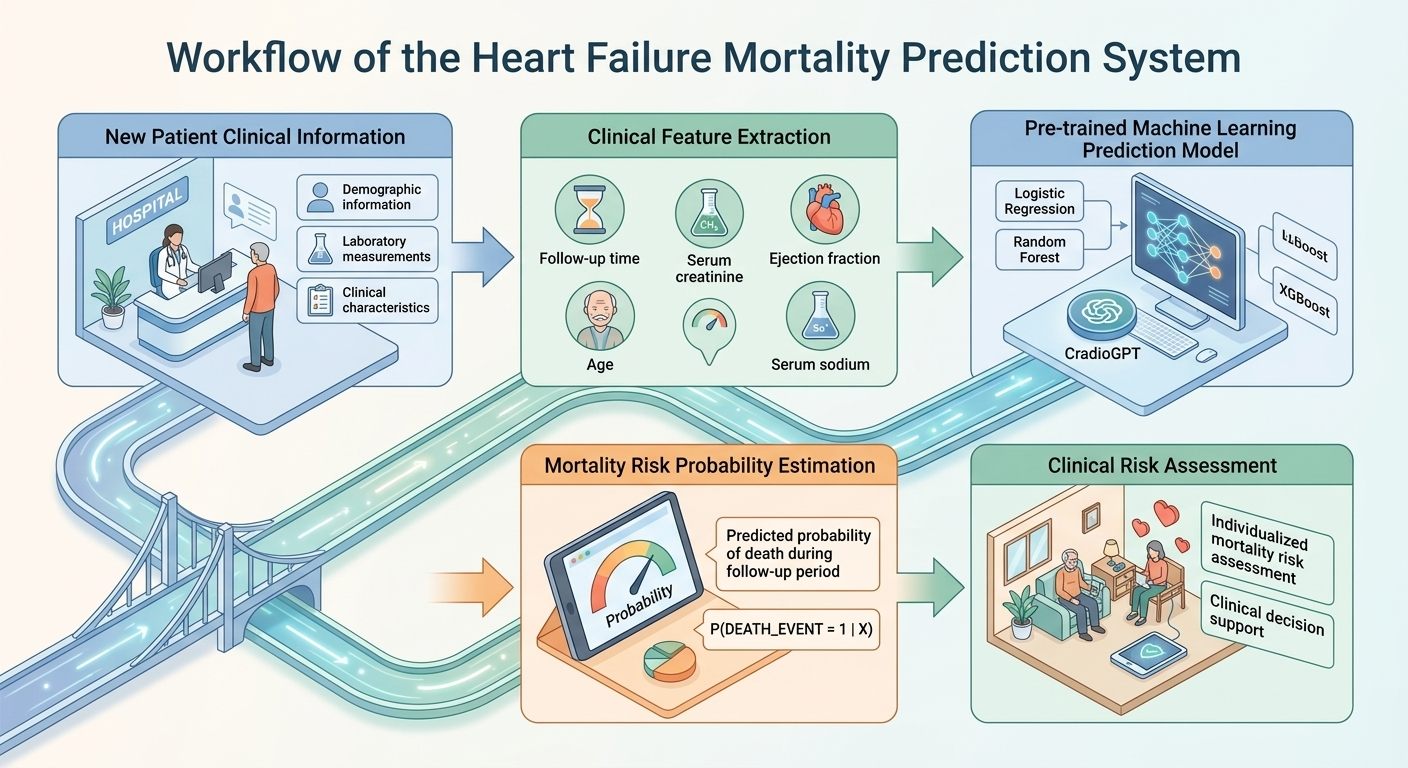
\includegraphics[width=0.85\linewidth]{workflow.png}
\caption{
Workflow of the proposed heart failure mortality prediction system.
}
\label{fig:workflow}
\end{figure}

%========================================================
\section{Results}


\subsection{Baseline Characteristics of Patients}


A total of 299 patients with heart failure were included in this study.
The baseline characteristics of the study population are summarized in
Table~\ref{tab:baseline}.

The mean age of the patients was 60.83 $\pm$ 11.89 years. The average
ejection fraction was 38.08 $\pm$ 11.83\%, and the mean serum creatinine level
was 1.39 $\pm$ 1.03 mg/dL. Among all patients, 96 (32.11\%) experienced death
during the follow-up period.



\begin{table}[H]
\centering
\caption{
Baseline characteristics of patients with heart failure.
}
\label{tab:baseline}

\begin{tabular}{lcc}
\toprule
Variable & Mean $\pm$ SD / n(\%) \\
\midrule

Age (years) & 60.83 $\pm$ 11.89 \\

Anaemia & 129 (43.14\%) \\

Creatinine phosphokinase & 581.84 $\pm$ 970.29 \\

Diabetes & 125 (41.81\%) \\

Ejection fraction (\%) & 38.08 $\pm$ 11.83 \\

High blood pressure & 105 (35.12\%) \\

Platelets & 263358.03 $\pm$ 97804.24 \\

Serum creatinine & 1.39 $\pm$ 1.03 \\

Serum sodium & 136.63 $\pm$ 4.41 \\

Male sex & 194 (64.88\%) \\

Smoking & 96 (32.11\%) \\

Follow-up time (days) & 130.26 $\pm$ 77.61 \\

Death event & 96 (32.11\%) \\

\bottomrule
\end{tabular}

\end{table}




%========================================================
\subsection{Identification of Mortality-Associated Factors}


Independent samples t-test and Spearman correlation analysis were performed
to identify clinical variables associated with mortality.

The correlation heatmap of the top 10 factors associated with
\textit{DEATH\_EVENT} is shown in Figure~\ref{fig:correlation}.


\begin{figure}[H]
\centering
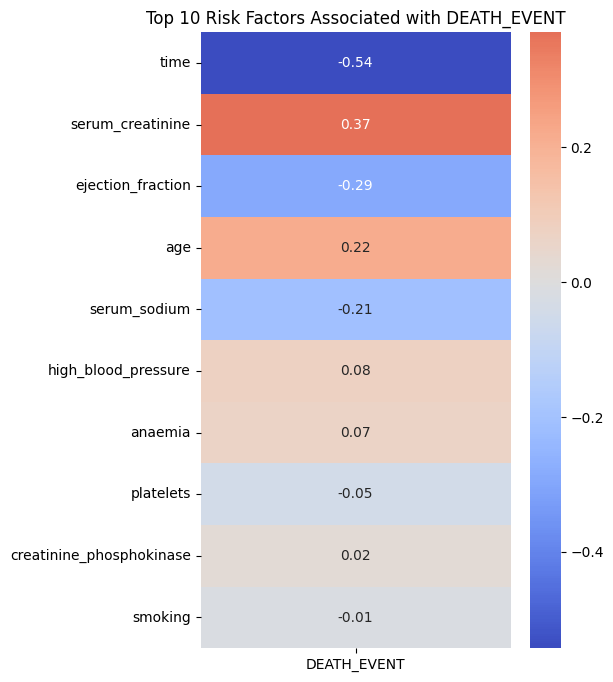
\includegraphics[width=0.65\linewidth]{correlation_heatma.png}

\caption{
Spearman correlation heatmap of clinical variables associated with
DEATH\_EVENT.
}

\label{fig:correlation}

\end{figure}



Among all evaluated variables, follow-up time showed the strongest correlation
with mortality outcome. Serum creatinine demonstrated a positive association
with mortality, indicating that impaired renal function may be related to poor
clinical outcomes. In contrast, ejection fraction and serum sodium showed
negative correlations, suggesting that reduced cardiac function and electrolyte
imbalance may contribute to increased mortality risk.



Based on the statistical analysis, five variables were selected as predictors:

\begin{itemize}

\item time

\item serum creatinine

\item ejection fraction

\item age

\item serum sodium

\end{itemize}




%========================================================
\subsection{Comparison of Machine Learning Models}


Three machine learning models were developed using the selected clinical
features. The performance comparison results are summarized in
Table~\ref{tab:model}.



\begin{table}[H]

\centering

\caption{
Performance comparison of different machine learning models.
}

\label{tab:model}


\begin{tabular}{lccccc}

\toprule

Model 
& Accuracy 
& Precision 
& Recall 
& F1-score 
& AUC \\

\midrule


Logistic Regression 
&0.833
&0.800
&0.632
&0.706
&0.890
\\


Random Forest
&0.817
&0.750
&0.632
&0.686
&0.900
\\


XGBoost
&0.850
&0.857
&0.632
&0.727
&0.873
\\


\bottomrule

\end{tabular}

\end{table}



Among the three models, XGBoost achieved the highest accuracy and F1-score,
indicating better classification performance in identifying patients with
mortality events. Random Forest obtained the highest AUC value (0.900),
suggesting superior discrimination ability between survival and mortality
groups. Logistic Regression showed competitive performance while maintaining
high interpretability.



\begin{figure}[H]

\centering

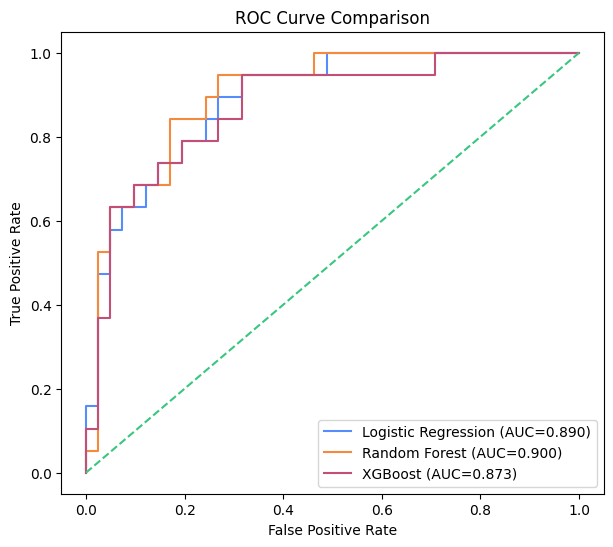
\includegraphics[width=0.65\linewidth]{ROC_compariso.png}


\caption{
ROC curves of Logistic Regression, Random Forest, and XGBoost models for
mortality prediction.
}

\label{fig:roc}

\end{figure}



%========================================================
\subsection{Clinical Application Workflow}


After comparing different machine learning models, the developed prediction
system can be applied to individual patients. The workflow consists of
inputting clinical characteristics, processing patient information through the
selected prediction model, and generating an estimated probability of mortality
during follow-up.

The workflow of the proposed prediction system is illustrated in
Figure~\ref{fig:workflow}.



%========================================================
\section{Discussion}


In this study, we developed a machine learning-based framework for predicting
mortality risk among patients with heart failure. By combining statistical
factor identification with machine learning algorithms, clinically meaningful
predictors were selected and used to estimate individual mortality probability.


The risk factor analysis identified several important variables associated with
mortality. Serum creatinine was positively associated with mortality risk,
which may reflect the influence of impaired renal function on heart failure
progression. The interaction between cardiac dysfunction and renal impairment,
often referred to as cardiorenal syndrome, has been recognized as an important
factor affecting prognosis in patients with heart failure.


Ejection fraction showed a negative association with mortality, indicating that
patients with reduced cardiac contractile function may experience increased
risk of adverse outcomes. Since ejection fraction is a widely used indicator of
left ventricular function, its inclusion in prediction models provides clinical
interpretability.


Age was also identified as an important predictor. Older patients generally
have increased cardiovascular burden and more frequent comorbidities, which may
contribute to increased mortality risk.


From the perspective of machine learning performance, XGBoost achieved the best
accuracy and F1-score, demonstrating its ability to capture complex patterns
within clinical data. Random Forest achieved the highest AUC, indicating strong
overall discrimination ability. Logistic Regression showed slightly lower
predictive performance but remained valuable due to its transparency and
interpretability, which are important considerations in clinical applications.


However, several limitations should be considered. First, this study was based
on a relatively small dataset with 299 patients, which may limit model
generalizability. Second, the variable time represented follow-up duration and
showed strong association with mortality; therefore, its application in real
clinical prediction requires careful consideration because it may introduce
information related to follow-up status. Future studies using larger
prospective cohorts are needed to validate the proposed approach.


%========================================================
\section{Conclusion}


This study developed and compared three machine learning models for predicting
mortality risk in patients with heart failure. Statistical analysis identified
important mortality-associated factors, including follow-up time, serum
creatinine, ejection fraction, age, and serum sodium. The developed models were
able to estimate individual mortality probability based on clinical
characteristics. Machine learning approaches may provide valuable support for
risk stratification and personalized management of patients with heart failure.

\newpage

%========================================================
\begin{thebibliography}{99}


\bibitem{heidenreich2022}
Heidenreich PA, Bozkurt B, Aguilar D, et al.
2022 AHA/ACC/HFSA Guideline for the Management of Heart Failure.
\textit{Circulation}. 2022.


\bibitem{mcDonagh2021}
McDonagh TA, Metra M, Adamo M, et al.
2021 ESC Guidelines for the diagnosis and treatment of acute and chronic heart failure.
\textit{European Heart Journal}. 2021.


\bibitem{chicco2020}
Chicco D, Jurman G.
Machine learning can predict survival of patients with heart failure from serum
creatinine and ejection fraction alone.
\textit{BMC Medical Informatics and Decision Making}. 2020.


\bibitem{breiman2001}
Breiman L.
Random forests.
\textit{Machine Learning}. 2001;45:5--32.


\bibitem{chen2016}
Chen T, Guestrin C.
XGBoost: A scalable tree boosting system.
In:
\textit{Proceedings of the 22nd ACM SIGKDD International Conference on Knowledge Discovery and Data Mining}.
2016.


\bibitem{hosmer2013}
Hosmer DW, Lemeshow S, Sturdivant RX.
\textit{Applied Logistic Regression}.
3rd ed.
Wiley; 2013.


\bibitem{konstam2017}
Konstam MA, Kiernan MS, Bernstein D, et al.
Evaluation and management of right-sided heart failure.
\textit{Circulation}. 2017.


\bibitem{ponikowski2016}
Ponikowski P, Voors AA, Anker SD, et al.
2016 ESC Guidelines for the diagnosis and treatment of acute and chronic heart failure.
\textit{European Heart Journal}. 2016.


\end{thebibliography}


\end{document}